\documentclass[12pt,letterpaper]{hmcpset}
\usepackage[margin=1in]{geometry}
\usepackage{graphicx}
\usepackage{amsmath,amssymb}
\usepackage{tikz}
\usetikzlibrary{decorations.pathmorphing,patterns}

% info for header block in upper right hand corner
\name{}
\class{ - Section ---}
\assignment{Work, Energy, and Dynamics}
\duedate{Monday, March 7, 2016}

\newcommand{\val}[2]{$#1$#2}

\begin{document}

\problemlist{5.12, 6.\{3,8,13\}}

\noindent
\textbf{Reading:} Chapters 5.6--5.11 and 6.1--6.3, 6.5

\begin{problem}[Lennard-Jones potential - KK 5.12]
  A commonly used potential energy function to describe the interaction between
  two atoms is the Lennard-Jones 6-12 potential given by
  \begin{equation*}
	U = \epsilon \left[ 
      \left( \frac{r_{0}}{r} \right)^{12} - 2 \left( \frac{r_{0}}{r} \right)^{6}
    \right]
  \end{equation*}
  \begin{enumerate}
    \item Find the position of the potential minimum and its value.
    \item Near the minimum the atoms execute simple harmonic motion. Find the
      frequency of oscillation.
  \end{enumerate}
\end{problem}

\begin{solution}
    \vfill
\end{solution}
\clearpage

\begin{problem}[Normal modes and symmetry - KK 6.3]

    Four identical masses $m$ are joined by 
    three identical springs, of spring constant
    $k$, and are constrained to move on a line,
    as shown. There is a high degree of symmetry
    in this problem, so that one can guess the normal mode
    motions by inspection, without a lengthy 
    calculation. Once the relative amplitudes of 
    the normal mode motions are known, the normal 
    mode vibrational frequencies follow directly.

    \begin{center}
    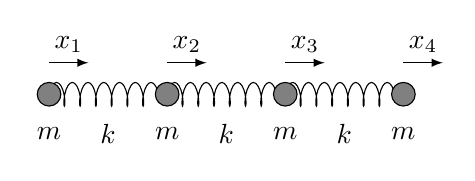
\begin{tikzpicture}[scale=1]
        \foreach \x in {0, 1.5, 3} {
            \draw[decoration={aspect=0.3, segment length=2mm, amplitude=1.5mm,coil},decorate] (\x,0) -- ++(0:1.5);
            \node at (\x+0.75, -0.5) {$k$};
        }
        \foreach \x in {1,2,3,4} {
            \filldraw[fill=gray] (1.5*\x-1.5,0) circle[radius=0.15]; 
            \node at (1.5*\x-1.5,-0.5) {$m$};
            \draw[-latex] (1.5*\x-1.5,0.4) -- node[anchor=south]{$x_{\x}$} ++ (0:0.5);
        }
    \end{tikzpicture}
    \end{center}

    Because of the symmetry, the normal mode 
    amplitudes must obey $x_{1} = \pm x_{4}$ 
    and $x_{2} = \pm x_{3}$. Another condition
    is that the center of mass must remain at
    rest. The possibilities are:

    \begin{enumerate}
        \item $(x_{4} = x_{1})$ and $(x_{3} = x_{2})$
        \item $(x_{4} = -x_{1})$ and $(x_{3} = -x_{2})$
    \end{enumerate}

    The normal mode equations lead to three 
    possible non-trivial vibrational frequencies
    and three corresponding normal modes. 
    Find the normal mode frequencies. It is 
    convenient to use the dimensionless parameter $\beta =
    \omega^{2}/\omega_{0}^{2}$, where $\omega$ is
    a frequency to be found and $\omega_{0} \equiv \sqrt{k/m}$.
\end{problem}

\begin{solution}
    \vfill
\end{solution}
\clearpage


\begin{problem}[Collision of $m$ and $M$ - KK 6.8]

    A particle of mass $m$ and initial velocity $v_{0}$
    collides elastically with a particle of unknown 
    mass $M$ coming from the opposite direction as shown in
    the sketch. After the collision, $m$ has velocity 
    $v_{0}/2$ at right angles to the incident direction, 
    and $M$ moves off in the direction shown in the
    sketch. Find the ratio $M/m$.

    \begin{center}
    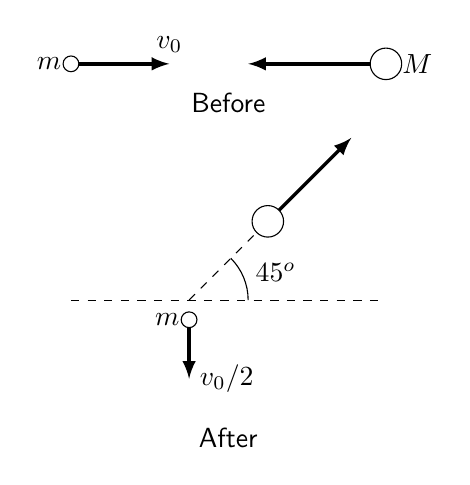
\begin{tikzpicture}[scale=1]
        \draw[very thick, -latex] (0,0) -- ++(0:1.25) node[anchor=south]{$v_{0}$};
        \draw[fill=white] (0,0) circle[radius=0.1] node[anchor=east]{$m$};
        \draw[very thick, -latex] (4,0) -- ++(180:1.75) ;
        \draw[fill=white] (4,0) circle[radius=0.2];
        \node at (4.4,0) {$M$};
        \node at (2,-0.5) {\textsf{Before}};

        \begin{scope}[shift={(0,-3)}]
            \draw (2.25,0) arc (0:45:0.75);
            \node at (2.6, 0.35){$45^o$};
            \draw[dashed] (0,0) -- (4,0);
            \draw[very thick, -latex] (1.5, -0.25) -- ++(-90:0.75) node[anchor=west]{$v_{0}/2$};
            \draw[fill=white] (1.5, -0.25) circle[radius=0.1]
            node[anchor=east]{$m$};
            \draw[dashed] (1.5,0) -- ++(45:1.5);
            \draw[very thick, -latex] (2.5,1) -- ++(45:1.5);
            \draw[fill=white] (2.5, 1) circle[radius=0.2];
            \node at (2, -1.75){\textsf{After}};
        \end{scope}
    \end{tikzpicture}
    \end{center}
\end{problem}

\begin{solution}
    \vfill
\end{solution}
\clearpage

\begin{problem}[Nuclear reaction of $\alpha$-rays with lithium - KK 6.13]
    A thin target of lithium is bombarded 
    by helium nuclei ($\alpha$-rays) of
    energy $E_{0}$. The lithium nuclei are 
    initially at rest in the target but are
    essentially unbound. When an $\alpha$-ray
    enters a lithium nucleus, a nuclear reaction
    can occur in which the compound nucleus 
    splits apart into a boron nucleus and a 
    neutron. The collision is inelastic, and
    the final kinetic energy is less than $E_{0}$
    by \val{2.8}{MeV}. The relative masses of the
    particles are: helium, mass 4; lithium, mass 7;
    boron, mass 10; neutron, mass 1. The reaction
    can be symbolized

    \[
        {}^7\text{Li} + {}^4\text{He} \longrightarrow {}^{10}\text{B} + {}^1\text{n} - 2.8\text{MeV}
    \]

    \begin{enumerate}
    \item What is $E_{0,\rm threshold}$, the minimum value
        of $E_{0}$ for which neutrons can be produced?
    \item Show that if the incident energy falls in the 
        range $E_{0,\rm threshold} < E_{0} <E_{0,\rm threshold}
        + 0.27\text{MeV}$, the neutrons ejected in the forward 
        direction do not all have the same energy but must
        have either one or the other of two possible energies.
        (You can understand the origin of the two groups by 
        looking at the reaction in the center of mass frame.)
    \end{enumerate}
\end{problem}

\begin{solution}
    \vfill
\end{solution}
\clearpage

\end{document}
